\chapter{Dimensionality Reduction}
\section{Theory}
Dimensionality reduction is used to reduce the number of variables of the feature extraction.
There is two methods to make Dimensionality reduction, the first method is Fisher's linear discriminant model.
Fisher's model takes a D-dimensional input vector \textbf{x} and project to one dimension bye the equation:
\begin{equation}
y = \mathbf{w}^T \mathbf{x}.
\label{eq:fisher}
\end{equation} 

The projection down to one dimension leads to loss of information, and the data even if it was well separated in D-dimensions, can become overlapping when only viewed in one dimension.
The other method is Principal component analysis (PCA), which can be used to make a dimensionality reduction of the dataset.
PCA works bye orthogonal project the of the data onto a lower dimensional linear space.
The new space is called principal subspace and are made so that the variance of the projected data is maximized. 

\begin{figure}[H]
\centering
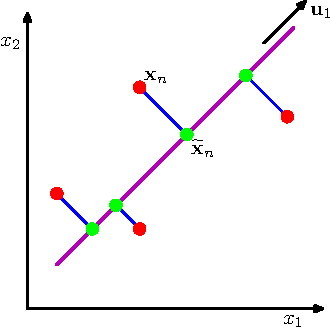
\includegraphics{Figure12_2_pdf}
\caption{Principal component analysis orthogonal project the of the data onto a lower dimensional linear space, This is shown on the figure. \fxnote{ref til bishop}}
\label{fig:dim_PCA_book}
\end{figure}

In this project PCA is used to make the dimensional reduction focusing on the maximum variance approach.

\subsection{Maximum Variance}
Consider a dataset of observations $ \left\lbrace \mathbf{x}_n \right\rbrace $ with $ n = 1,...,N $, and the data vector is a Euclidean variable with dimension D. 
The dataset can be projected to lower dimensional space with dimension $ M<D $ 	while maximizing the variance of the projected data. 



\section{Method}

\section{Results}

\subsection{Single digit:}

\subsection{Two digits:}

\subsection{Ten digits:}

\section{Discussion}

\fxnote{Diskuter resultater og evt forbedringer}